\FloatBarrier
\section{Messung} % (fold)
\label{sec:section_name}

Bei diesem Versuch werden zunächst die Leitungskonstanten drei verschiedener Kabel bestimmt, zwei RG 58C/U (10m,20m) und ein M17/028 RG 058 (100m).
Anschließend wird die Dämpfung des Signals untersucht, die Länge der Kabels bestimmt, die Leitungskonstanten auf andere Art und Weise berechnet, das Verhalten bei verschiedenen Abschlüssen untersucht und abschließend ein Impulsfahrplan einer Serienschaltung von verschiedenen Kabeln erstellt.

Im Folgenden wird für den Wellenwiderstand
\begin{equation}
	Z = \SI{50}{\ohm}
\end{equation}
angenommen.

Alle Fehler wurden mithilfe Gaußscher Fehlerfortpflanzung errechnet.
\begin{equation}
	\Delta f(x_\text{1}\text{,...,}x_\text{n}) = \sqrt{\sum_\text{i=0}^\text{n} \left(\frac{\partial f}{\partial x_\text{i}} \Delta x_\text{i}\right)^2}
\end{equation}
Dafür ist die Python Bibliothek \textit{uncertainties} benutzt worden.

Fehler wenn nicht anders angegeben:
\begin{eqnarray}
	U &=& +/-0.5\,[\text{mV}],\\
	f &=& +/-0.5\,[\text{kHz}],\\
	t &=& +/-5\,[\text{ns}].
\end{eqnarray}

\subsection{A: Leistungskonstanten verschiedener Kabel} % (fold)
\label{sub:a_}


Im ersten Teil werden die Leitungsparameter $R$, $L$, $C$ und $G$ der drei verschiedenen Kabel bestimmt.
$R$, $L$ und $C$ werden über ein Messgerät direkt gemessen, während $G$ über die Gleichung
\begin{equation}
	G = \frac{R C}{L}
\end{equation}
berechnet werden kann.
Die Ergebnisse sind den Tabellen \ref{tab_konst1} bis \ref{tab_konst3} zu entnehmen und die Leitungsparameter sind in Abhängigkeit der Frequenz in den Abbildungen \ref{fig_konst1} bis \ref{fig_konst4} dargestellt.


\begin{figure}
	\begin{minipage}{7.9cm}
		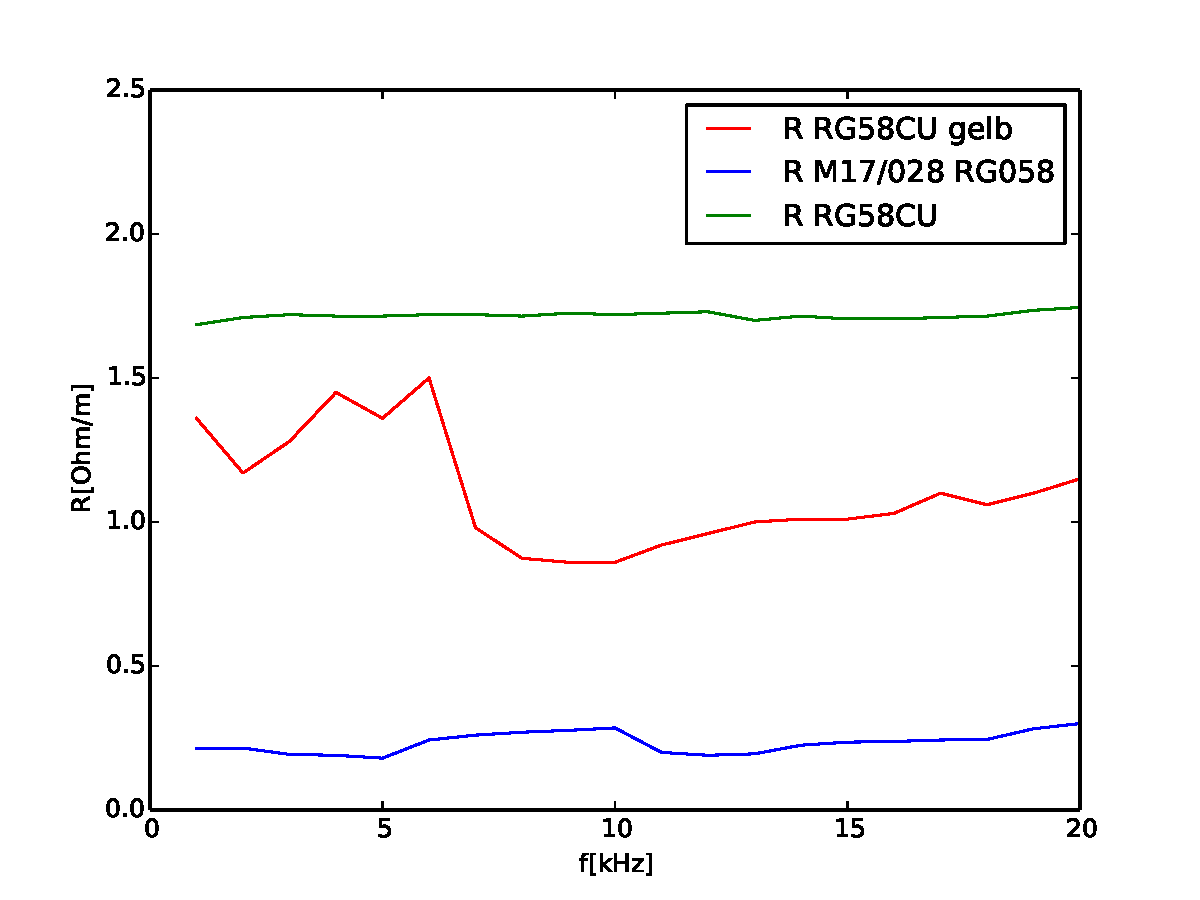
\includegraphics[width = 7.9cm]{data/a/R.pdf}
		\caption[]{Widerstandsbelag $R$ der verschiedenen ausgemessenen Kabel in Abhängigkeit der Frequenz.}
		\label{fig_konst1}
	\end{minipage}
	\begin{minipage}{7.9cm}
		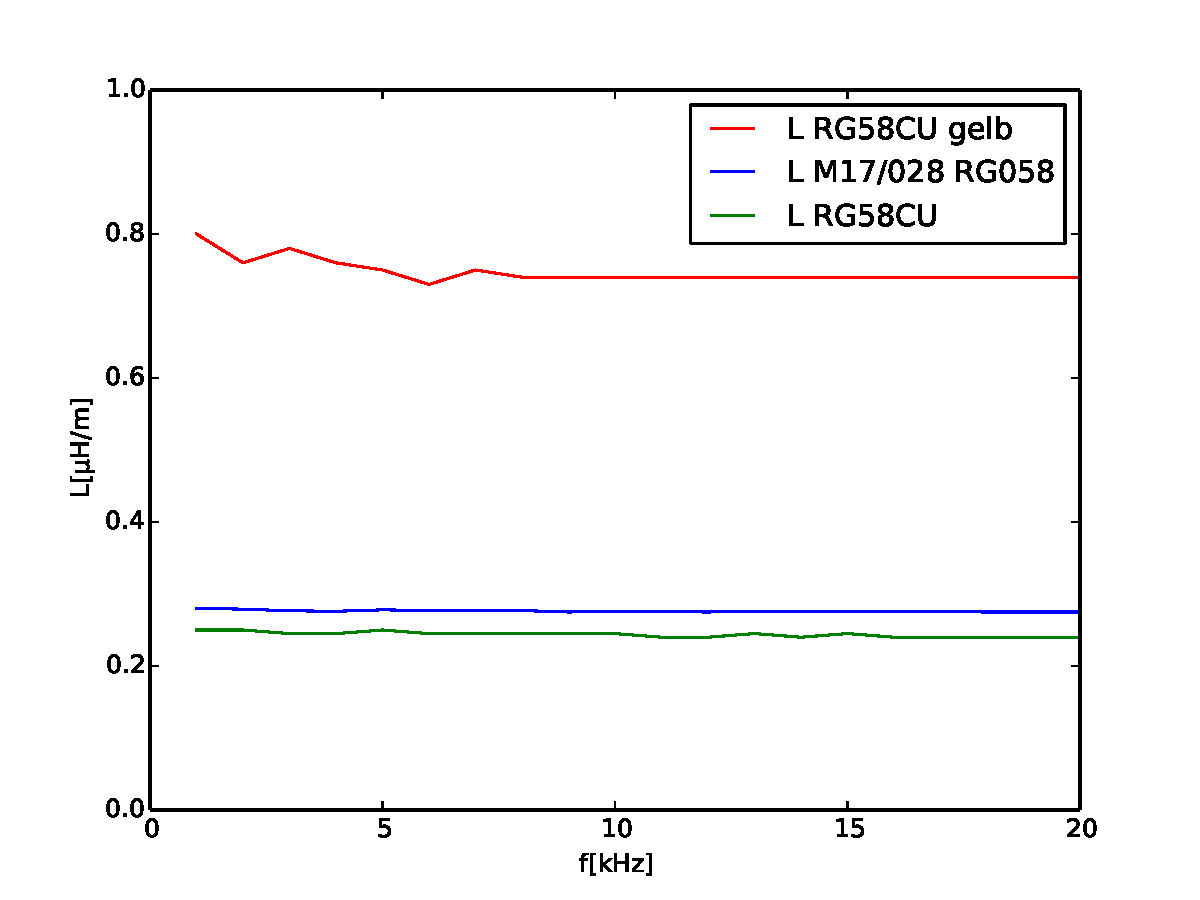
\includegraphics[width = 7.9cm]{data/a/L.pdf}
		\caption[]{Induktivitätsbelag $L$ der verschiedenen ausgemessenen Kabel in Abhängigkeit der Frequenz.}
		\label{fig_konst2}
	\end{minipage}
	\begin{minipage}{7.9cm}
		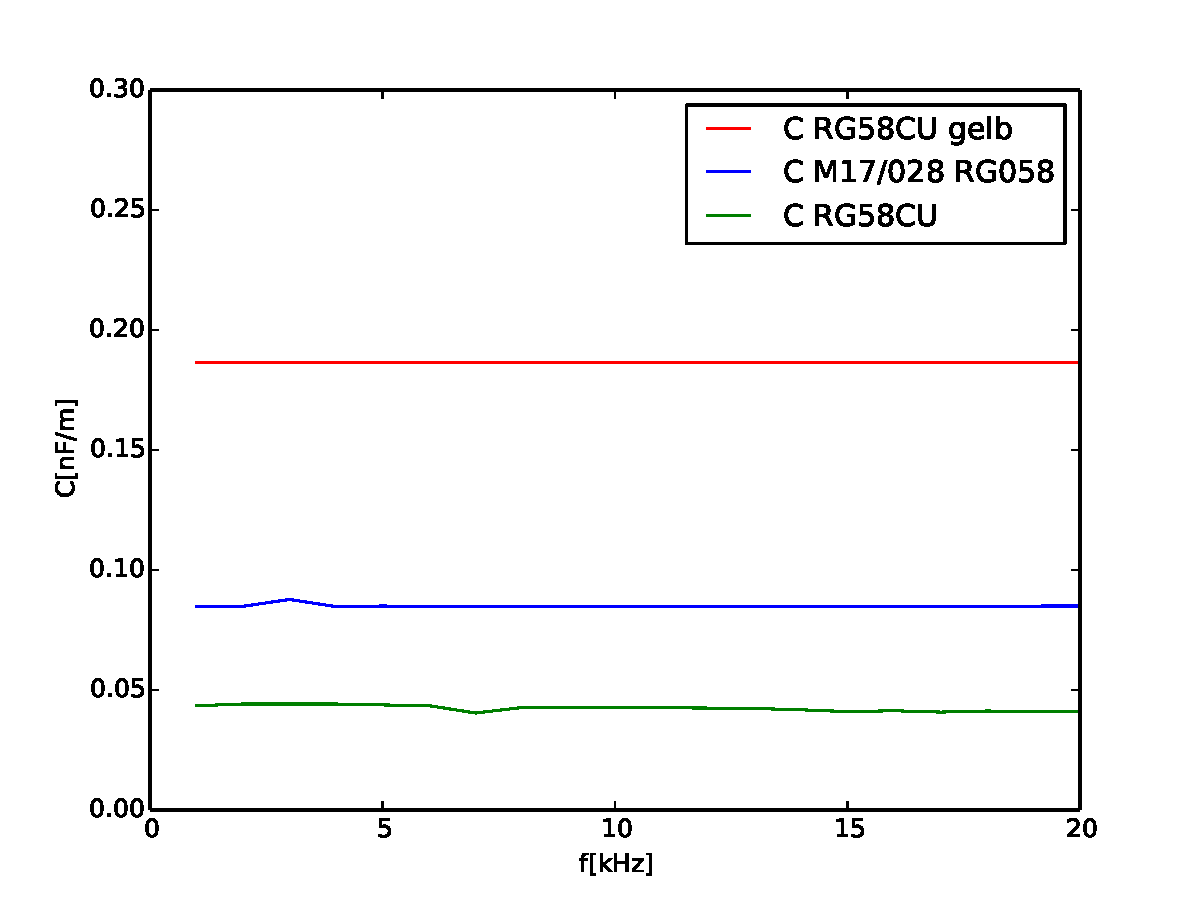
\includegraphics[width = 7.9cm]{data/a/C.pdf}
		\caption[]{Kapazitätsbelag $C$ der verschiedenen ausgemessenen Kabel in Abhängigkeit der Frequenz.}
		\label{fig_konst3}
	\end{minipage}
	\begin{minipage}{7.9cm}
		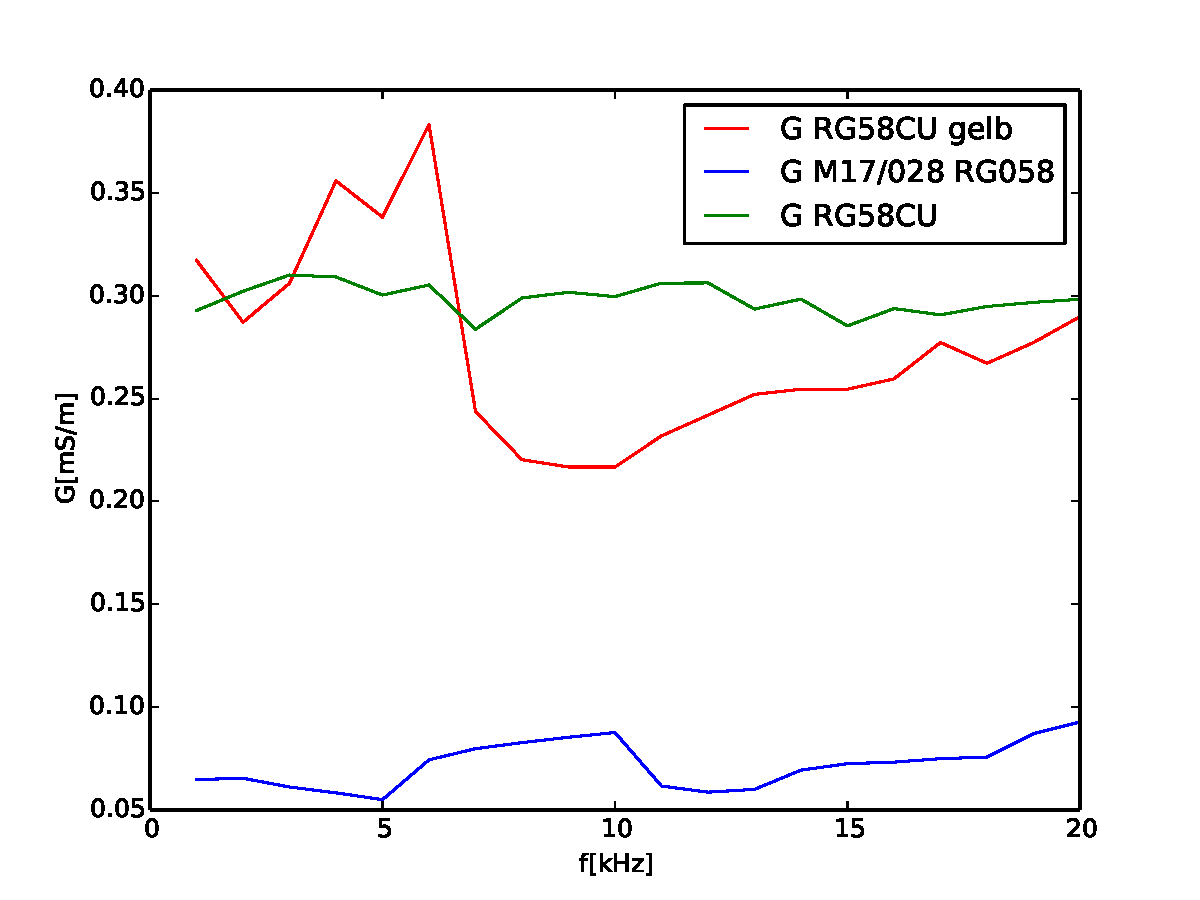
\includegraphics[width = 7.9cm]{data/a/G.pdf}
		\caption[]{Querleitwertbelag $G$ der verschiedenen ausgemessenen Kabel in Abhängigkeit der Frequenz.}
		\label{fig_konst4}
	\end{minipage}
\end{figure}

\begin{table}
\centering
	\caption[]{Leitungskonstanten des 10m RG 58C/U.}
	\begin{tabular}{r r r r r}
		f\,[kHz] & R\,[$\Omega$] & L\,[$\mu$H] & C\,[nF] & G\,[mS]\\
		\hline \hline
		  1	&	13.60	&	8.0	&	1.866	&	3.17\\
		  2	&	11.70	&	7.6	&	1.865	&	2.87\\
		  3	&	12.80	&	7.8	&	1.865	&	3.06\\
		  4	&	14.50	&	7.6	&	1.865	&	3.56\\
		  5	&	13.60	&	7.5	&	1.865	&	3.38\\
		  6	&	15.00	&	7.3	&	1.865	&	3.83\\
		  7	&	 9.80	&	7.5	&	1.865	&	2.44\\
		  8	&	 8.74	&	7.4	&	1.865	&	2.20\\
		  9	&	 8.60	&	7.4	&	1.865	&	2.17\\
		 10	&	 8.60	&	7.4	&	1.865	&	2.17\\
		 11	&	 9.20	&	7.4	&	1.865	&	2.32\\
		 12	&	 9.60	&	7.4	&	1.865	&	2.42\\
		 13	&	10.00	&	7.4	&	1.865	&	2.52\\
		 14	&	10.10	&	7.4	&	1.865	&	2.55\\
		 15	&	10.10	&	7.4	&	1.865	&	2.55\\
		 16	&	10.30	&	7.4	&	1.865	&	2.60\\
		 17	&	11.00	&	7.4	&	1.865	&	2.77\\
		 18	&	10.60	&	7.4	&	1.865	&	2.67\\
		 19	&	11.00	&	7.4	&	1.865	&	2.77\\
		 20	&	11.50	&	7.4	&	1.865	&	2.90\\
			\hline
	\end{tabular}
	\label{tab_konst1}
\end{table}

\begin{table}
\centering
	\caption[]{Leitungskonstanten des 20m RG 58C/U.}
	\begin{tabular}{r r r r r}
		f\,[kHz] & R\,[$\Omega$] & L\,[$\mu$H] & C\,[nF] & G\,[mS]\\
		\hline \hline
			  1	 &	33.7	&	5.0	&	0.8688	&	5.86\\
			  2	 &	34.2	&	5.0	&	0.8835	&	6.04\\
			  3	 &	34.4	&	4.9	&	0.8833	&	6.20\\
			  4	 &	34.3	&	4.9	&	0.8832	&	6.18\\
			  5	 &	34.3	&	5.0	&	0.8756	&	6.01\\
			  6	 &	34.4	&	4.9	&	0.8695	&	6.10\\
			  7	 &	34.4	&	4.9	&	0.8082	&	5.67\\
			  8	 &	34.3	&	4.9	&	0.8540	&	5.98\\
			  9	 &	34.5	&	4.9	&	0.8569	&	6.03\\
			 10  &	34.4	&	4.9	&	0.8534	&	5.99\\
			 11	 &	34.5	&	4.8	&	0.8518	&	6.12\\
			 12	 &	34.6	&	4.8	&	0.8496	&	6.12\\
			 13	 &	34.0	&	4.9	&	0.8460	&	5.87\\
			 14	 &	34.3	&	4.8	&	0.8350	&	5.97\\
			 15	 &	34.1	&	4.9	&	0.8200	&	5.71\\
			 16	 &	34.1	&	4.8	&	0.8270	&	5.88\\
			 17	 &	34.2	&	4.8	&	0.8160	&	5.81\\
			 18	 &	34.3	&	4.8	&	0.8250	&	5.90\\
			 19	 &	34.7	&	4.8	&	0.8210	&	5.94\\
			 20	 &	34.9	&	4.8	&	0.8205	&	5.97\\
			\hline
	\end{tabular}
	\label{tab_konst2}
\end{table}

\begin{table}
\centering
	\caption[]{Leitungskonstanten des 100m M17/028 RG 058.}
	\begin{tabular}{r r r r r}
		f\,[kHz] & R\,[$\Omega$] & L\,[$\mu$H] & C\,[nF] & G\,[mS]\\
		\hline \hline
			  1	&	21.38	&	28.00	&	8.488	&	6.48\\
			  2	&	21.50	&	27.90	&	8.488	&	6.54\\
			  3	&	19.30	&	27.67	&	8.772	&	6.12\\
			  4	&	19.00	&	27.60	&	8.474	&	5.83\\
			  5	&	18.00	&	27.80	&	8.500	&	5.50\\
			  6	&	24.30	&	27.70	&	8.480	&	7.44\\
			  7	&	26.00	&	27.65	&	8.488	&	7.98\\
			  8	&	27.00	&	27.70	&	8.489	&	8.27\\
			  9	&	27.65	&	27.50	&	8.489	&	8.54\\
			 10	&	28.50	&	27.60	&	8.490	&	8.77\\
			 11	&	20.00	&	27.55	&	8.491	&	6.16\\
			 12	&	19.00	&	27.50	&	8.493	&	5.87\\
			 13	&	19.50	&	27.60	&	8.495	&	6.00\\
			 14	&	22.50	&	27.55	&	8.495	&	6.94\\
			 15	&	23.56	&	27.60	&	8.495	&	7.25\\
			 16	&	23.80	&	27.60	&	8.496	&	7.33\\
			 17	&	24.30	&	27.55	&	8.497	&	7.49\\
			 18	&	24.50	&	27.50	&	8.498	&	7.57\\
			 19	&	28.20	&	27.50	&	8.498	&	8.71\\
			 20	&	30.01	&	27.50	&	8.500	&	9.28\\
			\hline
	\end{tabular}
	\label{tab_konst3}
\end{table}

\FloatBarrier
\subsection{B: Dämpfungskonstante} % (fold)
\label{sub:b_}

\begin{table}
\centering
	\caption[]{Dämpfungskonstanten des 100m M17/028 RG 058 Kabels.}
	\begin{tabular}{r r r r}
		f\,[kHz] & $U_0$\,[mV] & $U_\text{ged}$\,[mV] & $\alpha$\,[dB]\\
		\hline \hline
			79	&	92	&	89	&	0.66+/-0.16 \\
			88	&	86	&	83	&	0.71+/-0.17 \\
			96	&	80	&	77	&	0.76+/-0.18 \\
			106	&	74	&	71	&	0.83+/-0.20 \\
			115	&	67	&	64	&	0.92+/-0.22 \\
			124	&	60	&	59	&	0.34+/-0.24 \\
			133	&	56	&	54	&	0.73+/-0.26 \\
			143	&	52	&	50	&	0.78+/-0.28 \\
			151	&	49	&	47	&	0.83+/-0.29 \\
			160	&	45	&	44	&	0.45+/-0.32 \\
			170	&	41	&	41	&	0.00+/-0.34 \\
			179	&	40	&	39	&	0.50+/-0.40 \\
			188	&	38	&	37	&	0.50+/-0.40 \\
			196	&	36	&	35	&	0.60+/-0.40 \\
			205	&	35	&	33	&	1.20+/-0.40 \\
			214	&	33	&	32	&	0.60+/-0.40 \\
			224	&	32	&	30	&	1.30+/-0.50 \\
			233	&	31	&	29	&	1.30+/-0.50 \\
			241	&	30	&	28	&	1.40+/-0.50 \\
			251	&	28	&	27	&	0.70+/-0.50\\
			\hline
	\end{tabular}
	\label{tab_daempf}
\end{table}

In diesem Abschnitt werden die Dämpfungskonstanten eines 100m RG-58 C/U Kabels analysiert.
Dazu wurde zunächst ein Signal auf ein kurzes Kabel gegeben und die Amplituden $U_0$ der Oberwellenanteile bestimmt.
Anschließend wurde dasselbe Signal auf das lange Kabel gegeben um die Amplituden $U_\text{ged}$ der Oberwellen zu erhalten.
Anschließend kann die Dämpfungskonstante über
\begin{equation}
	\alpha = -20 \log \left( \frac{U_0}{U_\text{ged}}\right)
\end{equation}
berechnet werden.
Das Ergebnis und die verwendeten Werte sind in Tabelle \ref{tab_daempf} angegeben und in den Abbildungen \ref{fig_daempf1} und \ref{fig_daempf2} graphisch dargestellt.

\begin{figure}
	\centering
	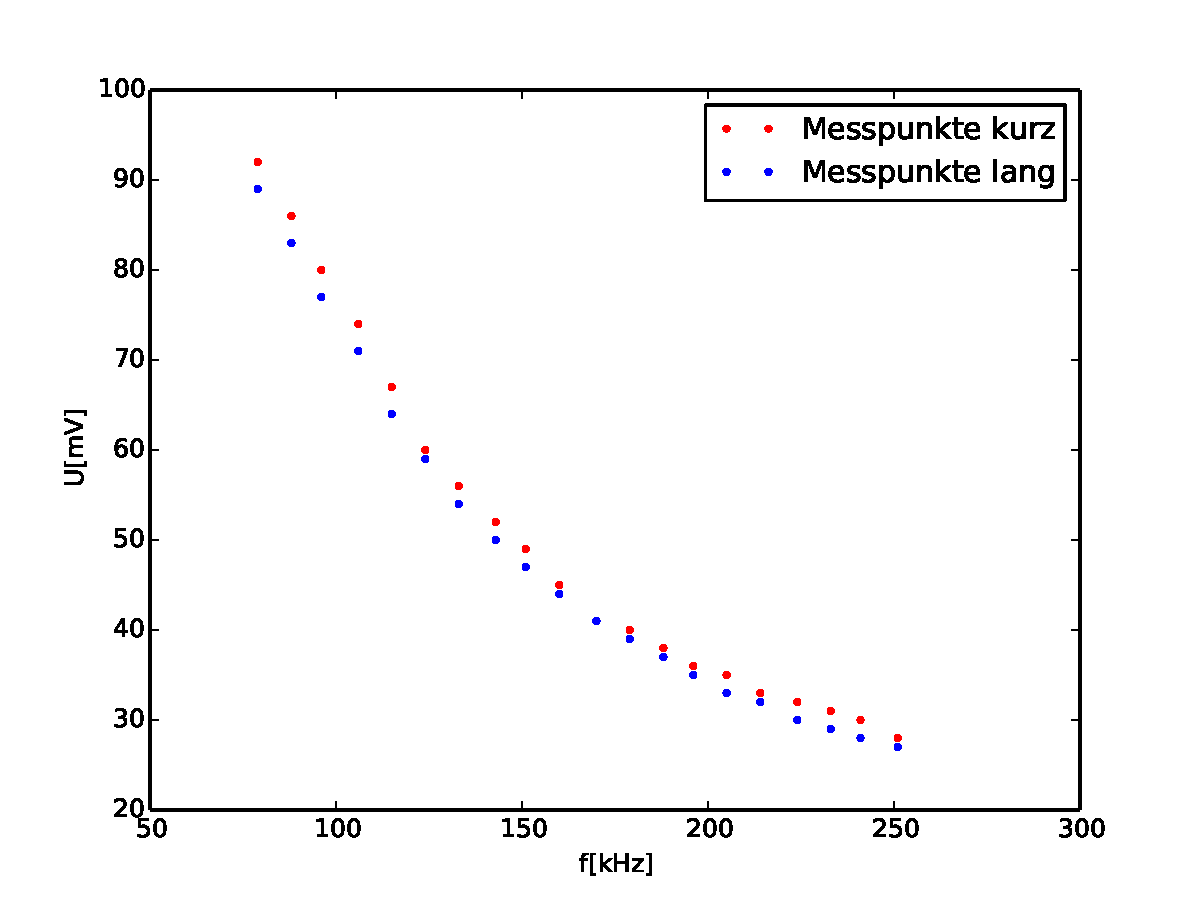
\includegraphics[width = 14cm]{data/b/alpha_zeit.pdf}
	\caption[]{Amplituden der Oberwellen des 100m M17/028 RG 058 Kabels und eines kurzen Kabels.}
	\label{fig_daempf1}
	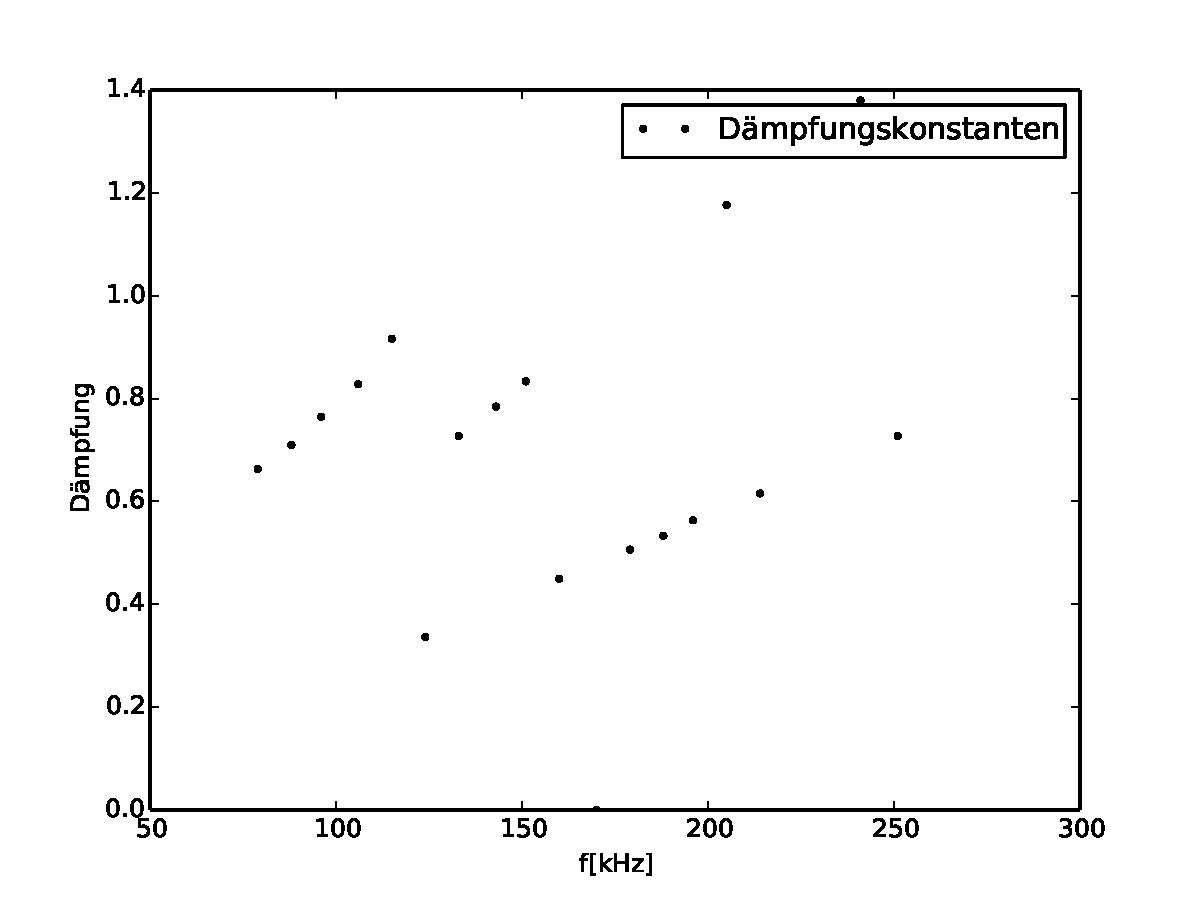
\includegraphics[width = 14cm]{data/b/alpha.pdf}
	\caption[]{Dämpfungskonstante des 100m M17/028 RG 058 Kabels in Abhängigkeit von der Frequenz.}
	\label{fig_daempf2}
\end{figure}

\FloatBarrier
\subsection{C: Spannungsverlauf bei offenem und geschlossenem Ende} % (fold)
\label{sub:c_laengenmessung}

\subsubsection{Bestimmung der Kabellänge durch Laufzeitmessung} % (fold)
\label{sub:bestimmung_der_kabellaenge_durch_laufzeitmessung}

Zur Bestimmung der Länge der verschiedenen Kabel wird auf die Laufzeit eines Strompulses zurückgegriffen.
Anhand der Spannungsverläufe lassen sich die Punkte $t_1$ und $t_2$ ablesen, an denen der Anfangspuls und der reflektierte Strompuls beginnen.
Zunächst wird die Differenz der beiden Zeiten gebildet, um daraus mithilfe der Gleichung
\begin{equation}
	l = \frac{v \Delta t}{2}
\end{equation}
die Länge $l$ zu berechnen.
Die Geschwindigkeit $v$ ist dabei zu
\begin{equation}
	v = c/\sqrt{\epsilon_r} \approx 2*10^{8}\,\frac{\text{m}}{\text{s}}
\end{equation}
bestimmt worden.
Die gemessenen und bestimmten Daten sind in Tabelle \ref{tab_zeit1} dargestellt.


\begin{table}
\centering
	\caption[]{Zur Längenbestimmung genutzte Zeiten und die resultierenden Ergebnisse.}
	\begin{tabular}{r r r r r}
		Kabel & $t_1$\,[ns] & $t_2$\,[ns] & $\Delta t$\,[100 ns] & l\,[m]\\
		\hline \hline
		 RG 58C/U & & & & \\
		 offen & 	  25.4	&   -85.0	&	 1.10+/-0.07 &	 10.93+/-0.70\\
		geschlossen	& 125.1	&     0.1	&	 1.25+/-0.07 &	 12.38+/-0.70\\
		RG 58C/U & &&&\\
		geschlossen	&  -0.0	&  1081.0	&	10.81+/-0.07 &	107.02+/-0.70\\
		offen	 & 118.0	&  -810.0	&	 9.28+/-0.07 &	 91.87+/-0.70\\
		M17/028 RG 058&&&&\\
		offen 	 & 19.0	&   209.0	&	 1.90+/-0.07 &	 18.81+/-0.70\\
		geschlossen	 & -12.6	&   195.6	&	 2.08+/-0.07 &	 20.61+/-0.70\\
			\hline
	\end{tabular}
	\label{tab_zeit1}
\end{table}
\FloatBarrier
\subsubsection{Bestimmung der Leitungskonstanten anhand der Spannungsverläufe} % (fold)
\label{sub:bestimmung_der_kabellaenge_anhand_der_spannungsverlaeufe}

Die Leitungskonstanten konnten nur Anhand des 100m Kabels mithilfe der Spannungsverläufe (Abbildungen \ref{fig_zeit1} bis \ref{fig_zeit3}) bestimmt werden, da ansonsten der induktive und kapazitive Anteil nicht zu erkennen ist.
Zunächst wurde dafür aus der Abbildung die Spannung der drei sichtbaren Plateaus über Mittelung der Werte berechnet, woraus sich nach suptraktion der Nullspannung $U_0$ die Werte
\begin{eqnarray}
	U_{0_\text{offen}} &=& \SI{-24.46(5)}{\volt},\\
	U_{1_\text{offen}} &=& \SI{37.94(5)}{\volt},\\
	U_{2_\text{offen}} &=& \SI{47.49(7)}{\volt},\\
	U_{0_\text{gesch}} &=& \SI{-2.59(5)}{\volt},\\
	U_{1_\text{gesch}} &=& \SI{25.01(6)}{\volt},\\
	U_{2_\text{gesch}} &=& \SI{5.98(7)}{\volt}
\end{eqnarray}
ergaben.

Der Reflexionsfaktor $\Gamma$ lässt sich daraus mithilfe der Gleichung
\begin{equation}
	U_1 (1+\Gamma) = U_2,
\end{equation}
 berechnen.
Damit ergiebt sich
\begin{eqnarray}
	\Gamma_\text{offen} &=& \SI{0.2517(15)}{},\\
	\Gamma_\text{gesch} &=& \SI{-0.7509(25)}{}.
\end{eqnarray}

Mithilfe des Reflexionsfaktors lässt sich mit $Z=\SI{50}{\ohm}$ aus der Gleichung
\begin{equation}
	\Gamma = \frac{R-Z}{R+Z}
\end{equation}
der Widerstandsbelag $R$ berechnen.
Damit ergiebt sich
\begin{eqnarray}
	R_\text{offen} &=& \SI{83.63(26)}{\ohm},\\
	R_\text{gesch} &=& \SI{6.79(8)}{\ohm}.
\end{eqnarray}

Um den Induktivitätsbelag $L$ berechnen zu können wird angenommen, dass bei einem $RL$ Abschluss in Serienschaltung der reflektierte elektrische Puls einen exponentiellen Zusammenhang besitzt.
Die Zeitkonstante der Funktion ist somit durch die Gleichung
\begin{equation}
	\tau_{RL} = \frac{L}{Z+R}
\end{equation}
gegeben.
Um an den negativen reziproken Wert der Zeitkonstanten zu gelangen, sind die Werte in diesem Bereich logarithmiert worden.
Mithilfe einer linearen Regression mit $f(x)=mx+b$ (Abbildung \ref{fig_fit1})hat sich für die Steigung
\begin{eqnarray}
	m_\text{offen} &=& \SI{-7.89(30)e5}{1\per\second},\\
	m_\text{gesch} &=& \SI{-2.60(2)e7}{1\per\second},
\end{eqnarray}
ergeben und somit für den Induktivbelag
\begin{eqnarray}
	L_\text{gesch} &=& \SI{169.00(6)}{\micro\henry}.
\end{eqnarray}

Mithilfe der Gleichung
\begin{eqnarray}
	C = -\frac{1}{mZ}
\end{eqnarray}
kann zudem der Kapazitivbelag $C$ berechnet werden.
Für diesen ergiebt sich somit
\begin{eqnarray}
	C_\text{offen} &=& \SI{2.53(9)e-8}{\farad}.
\end{eqnarray}

\begin{figure}
	\centering
	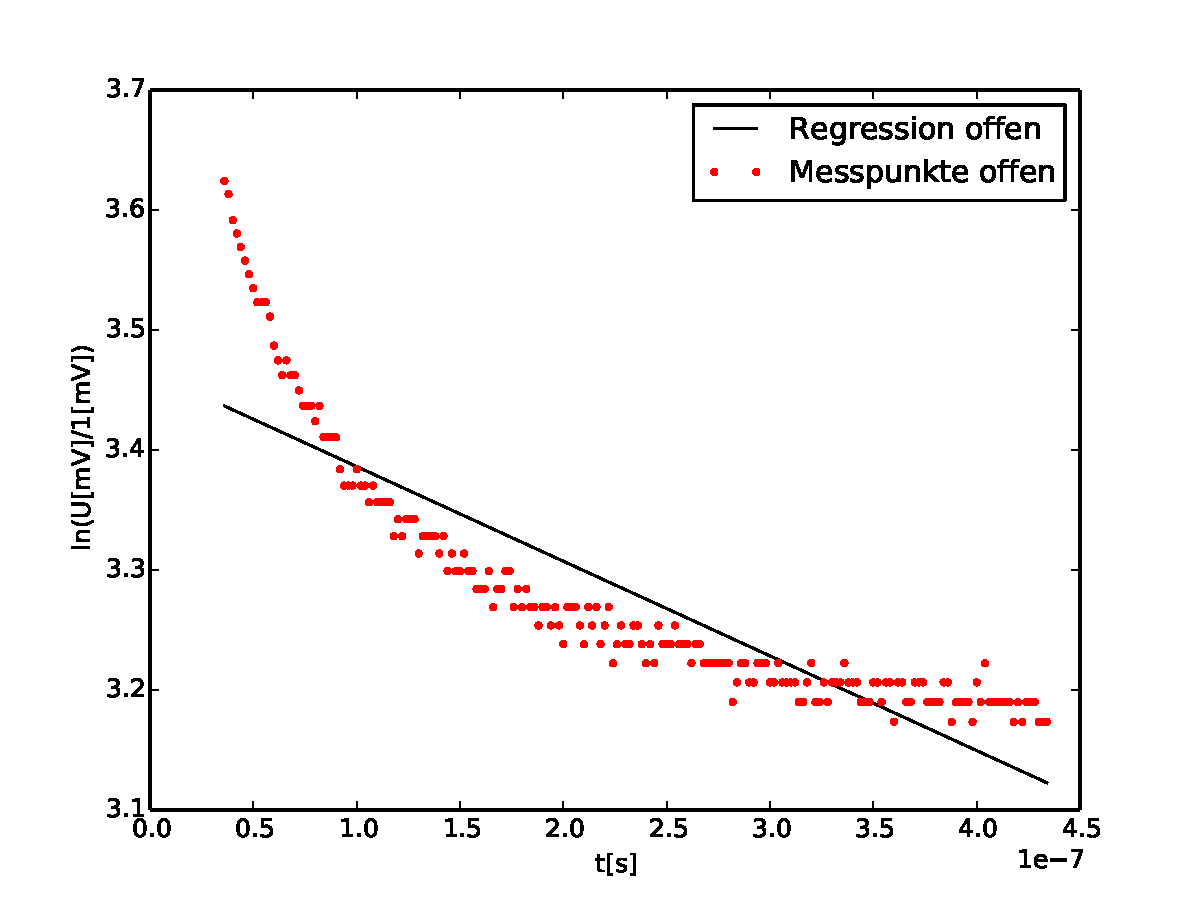
\includegraphics[width = 14cm]{data/c/Regression1.pdf}
	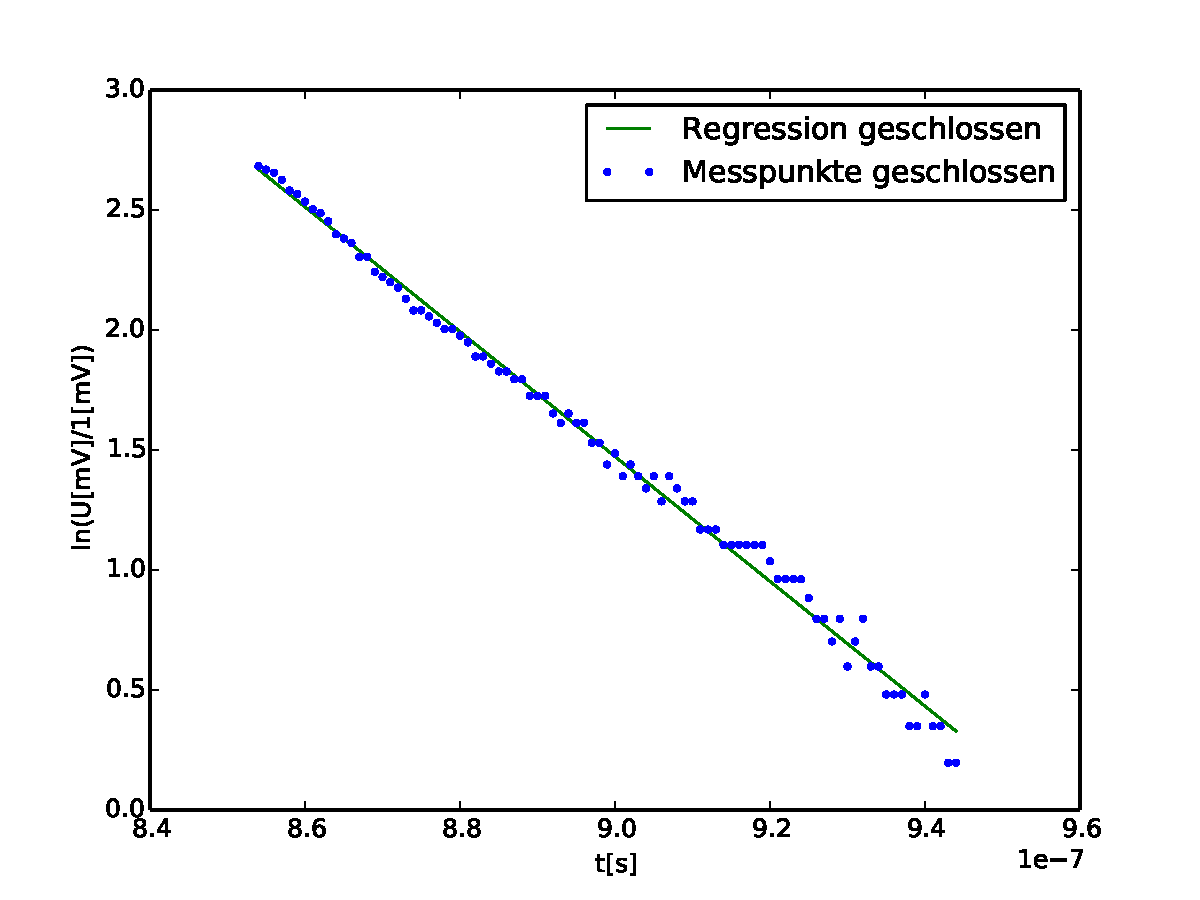
\includegraphics[width = 14cm]{data/c/Regression2.pdf}
	\caption{Lineare Ausgleichsrechnungen zur Bestimmung des Induktivbelages und des Kapazitivbelags.}
	\label{fig_fit1}
\end{figure}
\begin{figure}
\centering
	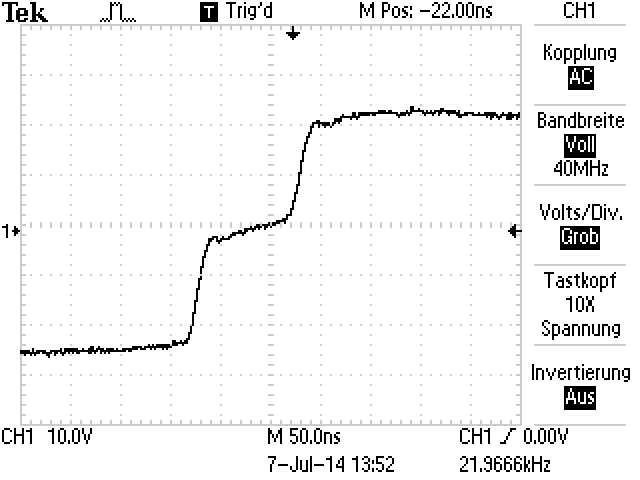
\includegraphics[width = 12cm]{data/c/ALL0000/F0000TEK.jpg}
	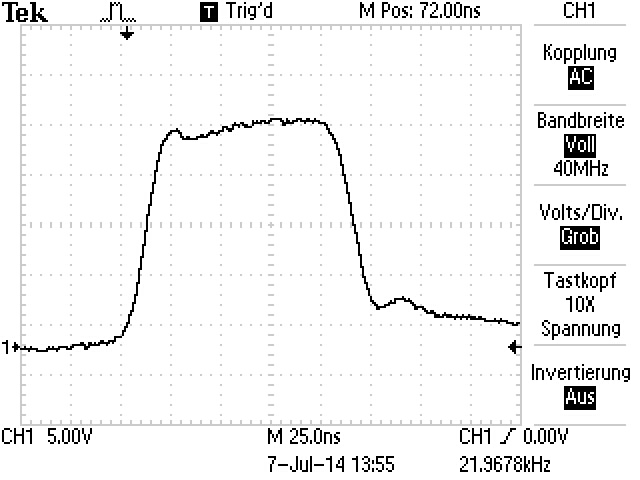
\includegraphics[width = 12cm]{data/c/ALL0001/F0001TEK.jpg}
	\caption{Spannungsverlauf eines RG 58C/U Kabels.}
	\label{fig_zeit1}
\end{figure}
\begin{figure}
\centering
	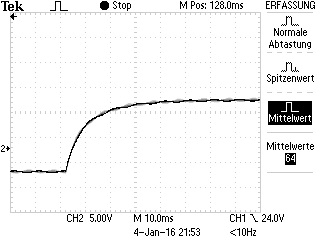
\includegraphics[width = 12cm]{data/c/ALL0002/F0002TEK.jpg}
	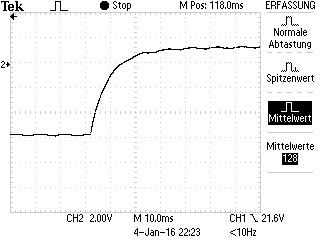
\includegraphics[width = 12cm]{data/c/ALL0003/F0003TEK.jpg}
	\caption{Spannungsverlauf eines M17/028 RG 058 Kabels.}
	\label{fig_zeit2}
\end{figure}
\begin{figure}
\centering
	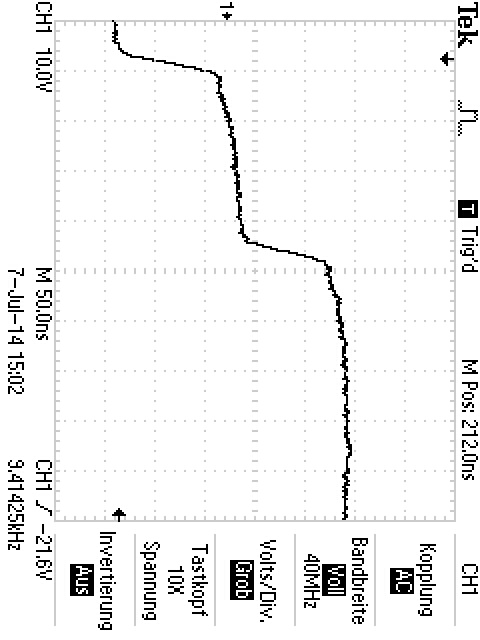
\includegraphics[width = 12cm]{data/c/ALL0011/F0011TEK.jpg}
	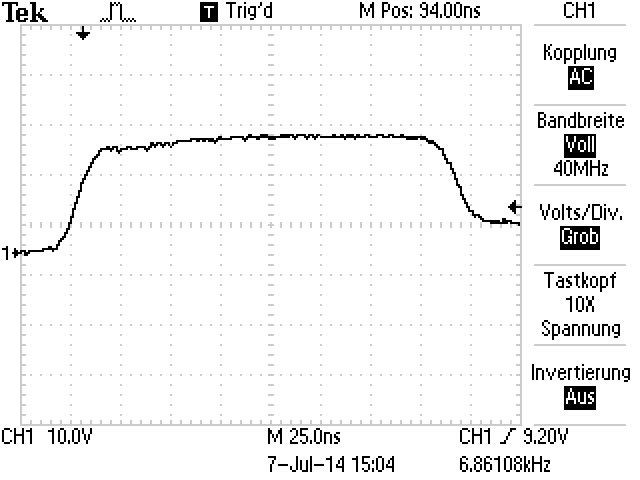
\includegraphics[width = 12cm]{data/c/ALL0012/F0012TEK.jpg}
	\caption{Spannungsverlauf eines RG 58C/U Kabels.}
	\label{fig_zeit3}
\end{figure}

\FloatBarrier
\subsubsection{Bestimmung der Kabellänge mithilfe eines Smith-Diagramms} % (fold)
\label{sub:bestimmung_der_kabellaenge_mithilfe_eines_smith_diagramms}

Um die Kabellänge mit einem Smith-Diagramm bestimmen zu können, muss zunächst die transformierte Impedanz 
\begin{equation}
	Z_L = R + i 2 \pi f L
\end{equation}
bekannt sein.
Mithilfe der errechneten Werte aus Kapitel \ref{sub:bestimmung_der_kabellaenge_anhand_der_spannungsverlaeufe} und einer Frequenz von $\SI{1}{\kilo\hertz}$ ist diese
\begin{eqnarray}
	Z_{L_\text{gesch}} &=& 6.79 + 0.01i.
\end{eqnarray}

Der Reflexionsfaktor $\Gamma_L$ lässt sich mithilfe der Gleichung
\begin{equation}
	\Gamma_L = \frac{Z_L-Z}{Z_L+Z}
\end{equation}
bestimmen, womit sich
\begin{eqnarray}
	\Gamma_{L_\text{gesch}} &=& -0.7609 + 0.0004i
\end{eqnarray}
ergiebt.

Der Winkel der komplexen Ebene zwischen dem Reflexionsfaktor $\Gamma_L$ und dem alten Reflexionsfaktor $\Gamma_A$ aus Kapitel \ref{sub:bestimmung_der_kabellaenge_anhand_der_spannungsverlaeufe} lässt sich durch
\begin{equation}
	\Theta = \arccos \left(\frac{\vec{\Gamma_L}\vec{\Gamma_L}}{|\vec{\Gamma_L}||\vec{\Gamma_L}|}\right)
\end{equation}
bestimmen.
Somit ergiebt sich
\begin{eqnarray}
	\Theta_\text{gesch} &\approx& 0.0056.
\end{eqnarray}

Daraus lässt sich gemäß der Gleichung
\begin{equation}
	l = \frac{c \Theta}{4 \pi f \sqrt{\epsilon_r}}
\end{equation}
die Länge des Kabels errechnen.
Es ergiebt sich
\begin{eqnarray}
	l_\text{gesch} &\approx& \SI{8.90}{\meter}.
\end{eqnarray}

Zudem kann die Länge über die Kapazität bestimmt werden mit
\begin{equation}
	Z_L = -\frac{i}{2 \pi f C}
\end{equation}
und $\Gamma_A = 1$.
Damit ergab sich nach analoger Rechnung für die Länge
\begin{eqnarray}
	l_\text{offen} &\approx& \SI{253.47}{\meter}.
\end{eqnarray}

\FloatBarrier
\subsection{D: Spannungsverlauf verschiedener Abschlusswiderstände} % (fold)
\label{sub:spannungsverlauf_verschiedener_abschlusswiderstaende}

Die relative Dielektrizitätskonstante $\epsilon_r$ berechnet sich aus dem Kapazitätsbelag $C$, dem Induktivbelages $L$ und dem inneren und äußeren Durchmesser des Koaxialkabels $d$ und $D$ durch
\begin{equation}
	\epsilon_r = \left(\frac{\sqrt{\frac{L}{C}}}{\log{\frac{D}{d}} \SI{60}{\ohm}}\right)^{-2}. \text{[koax]} 
\end{equation}

Dabei ist über die erhaltenen Größen von $C$ gemittelt worden.
Es ergab sich
\begin{equation}
	\epsilon_r = \SI{4.35(11)}{\farad\per\meter}.
\end{equation}

\subsubsection{Abschluss 1} % (fold)
\label{sub:abschluss_1}

Der Spannungsverlauf von Abschluss 1 ist in Abbildung \ref{fig_abs1} dargestellt.
Anhand der der Anleitung beigelegten Spannungsverläufe handelt es sich hierbei um einen RC-Serien\-schaltungs Abschluss.


\begin{table}
\centering
	\caption[]{Ergebnisse der Leitungskonstanten von Abschluss 1.}
	\begin{tabular}{r|r}
		\hline\hline
		$U_0$    & $\SI{-24.22(5)}{\volt}$\\
		$U_1$    & $\SI{25.83(5)}{\volt}$\\
		$U_2$    & $\SI{46.81(5)}{\volt}$\\
		$\Gamma$ & $\SI{0.812(5)}{}$\\
		$R$    & $\SI{482.7(151)}{\ohm}$\\
		m      & $\SI{-3.67(4)e4}{1\per\second}$\\
		$C$    & $\SI{5.12(16)e-8}{\farad}$\\
	\end{tabular}
\end{table}

\begin{figure}
	\centering
	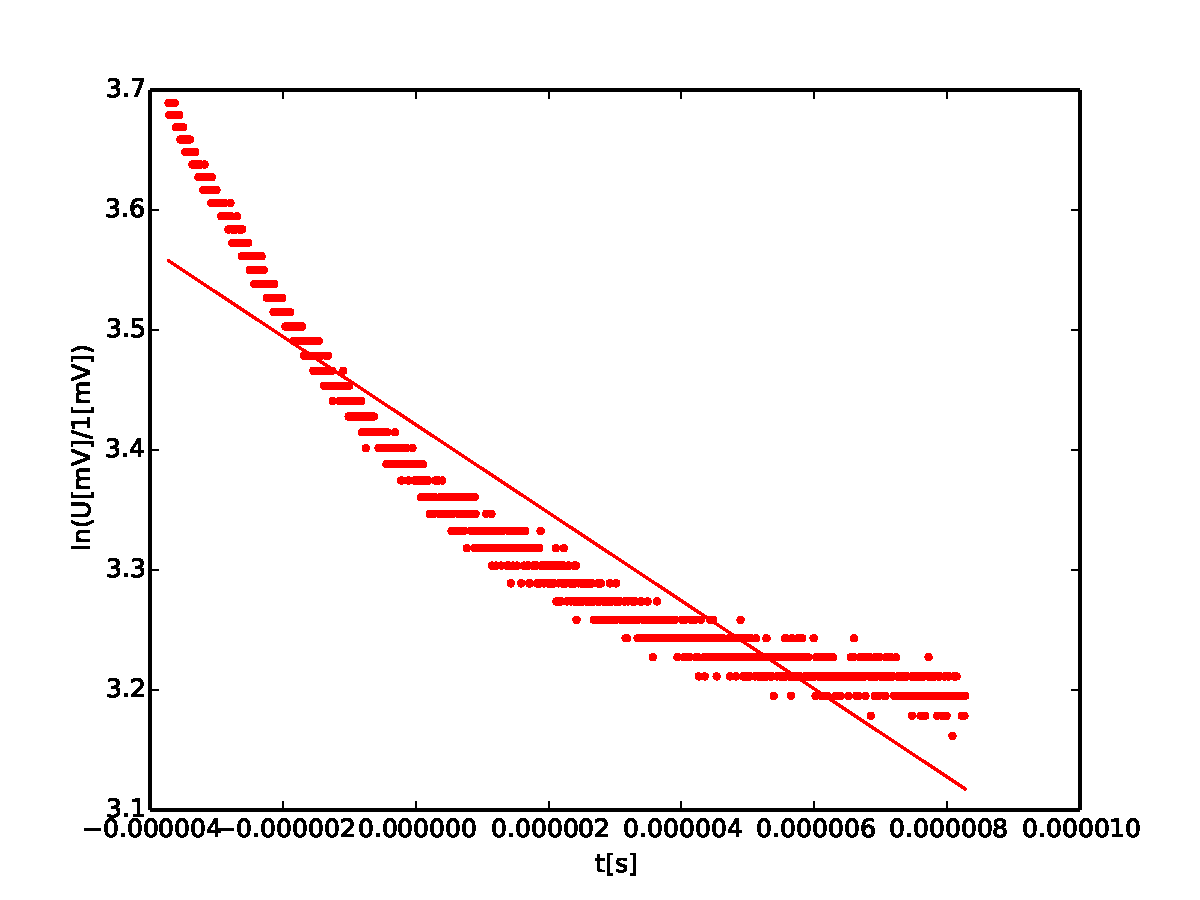
\includegraphics[width = 14cm]{data/d/Regression1.pdf}
	\caption{Lineare Ausgleichsrechnungen zur Bestimmung des Induktivbelages und des Kapazitivbelags.}
	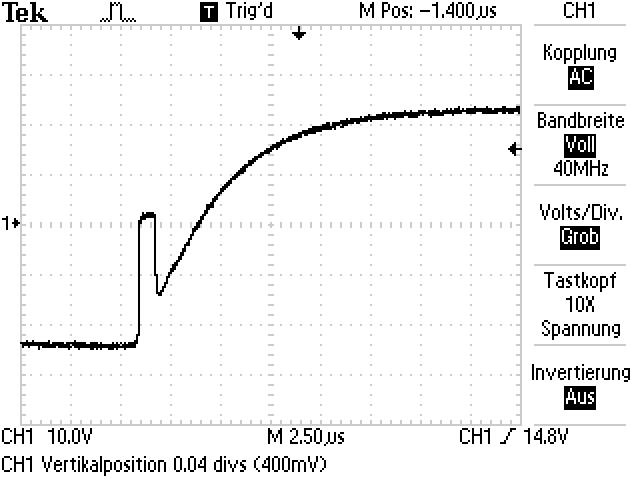
\includegraphics[width = 12cm]{data/d/F0004TEK.JPG}
	\caption{Spannungsverlauf von Abschluss 1.}
	\label{fig_abs1}
\end{figure}

\subsubsection{Abschluss 4} % (fold)
\label{sub:abschluss_4}

Der Spannungsverlauf von Abschluss 4 ist in Abbildung \ref{fig_abs4} dargestellt.
Anhand der der Anleitung beigelegten Spannungsverläufe handelt es sich hierbei um einen RL-Serien\-schaltungs Abschluss.

\begin{table}
\centering
	\caption[]{Ergebnisse der Leitungskonstanten von Abschluss 4.}
	\begin{tabular}{r|r}
		\hline\hline
		$U_0$    & $\SI{-3.33(5)}{\volt}$\\
		$U_1$    & $\SI{25.89(6)}{\volt}$\\
		$U_2$    & $\SI{6.86(7)}{\volt}$\\
		$\Gamma$ & $\SI{-0.7350(24)}{}$\\
		$R$    & $\SI{7.64(8)}{\ohm}$\\
		m      & $\SI{-6.576(34)e5}{1\per\second}$\\
		$L$    & $\SI{8.76(5)e-5}{\henry}$\\
	\end{tabular}
\end{table}

\begin{figure}
	\centering
	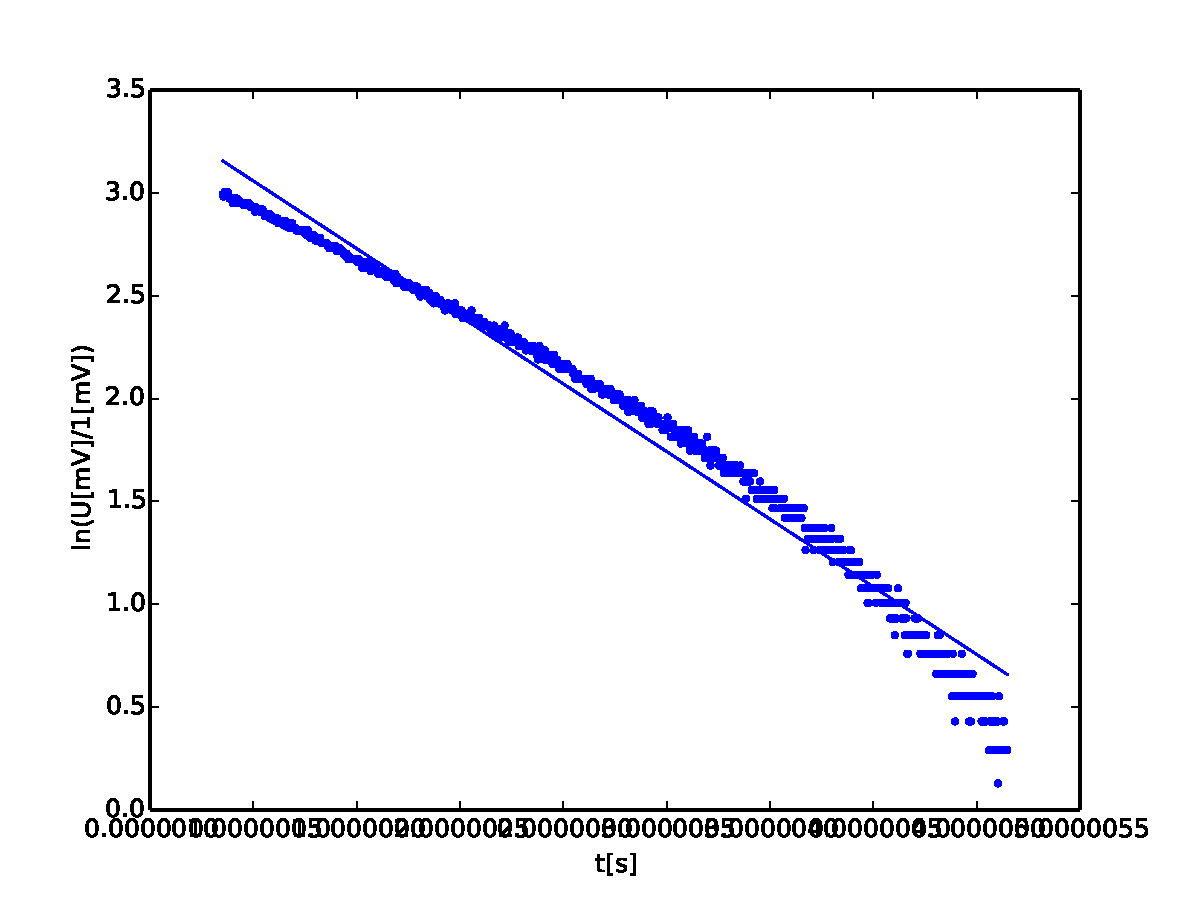
\includegraphics[width = 14cm]{data/d/Regression2.pdf}
	\caption{Lineare Ausgleichsrechnungen zur Bestimmung des Induktivbelages und des Kapazitivbelags.}
	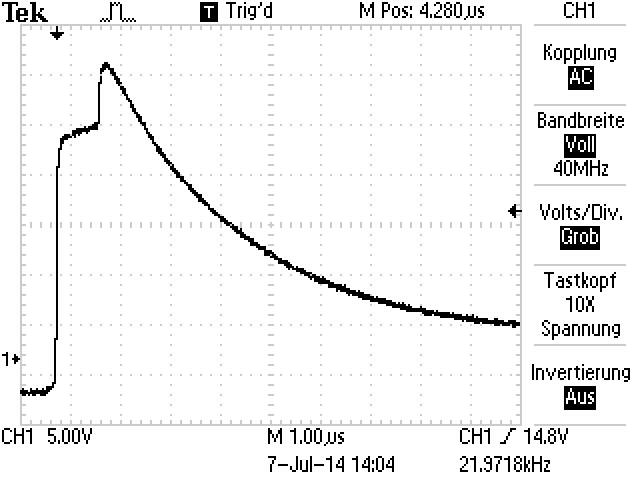
\includegraphics[width = 12cm]{data/d/F0005TEK.JPG}
	\caption{Spannungsverlauf von Abschluss 4.}
	\label{fig_abs4}
\end{figure}
\subsubsection{Abschluss 10} % (fold)
\label{sub:abschluss_10}

Der Spannungsverlauf von Abschluss 10 ist in Abbildung \ref{fig_abs10} dargestellt.
Anhand der der Anleitung beigelegten Spannungsverläufe handelt es sich hierbei um einen RC-Serien\-schaltungs Abschluss.

\begin{table}
\centering
	\caption[]{Ergebnisse der Leitungskonstanten von Abschluss 10.}
	\begin{tabular}{r|r}
		\hline\hline
		$U_0$    & $\SI{-18.16(5)}{\volt}$\\
		$U_1$    & $\SI{25.96(5)}{\volt}$\\
		$U_2$    & $\SI{34.69(7)}{\volt}$\\
		$\Gamma$ & $\SI{0.3365(22)}{}$\\
		$R$    & $\SI{100.7(5)}{\ohm}$\\
		m      & $\SI{-6.69(23)e4}{1\per\second}$\\
		$C$    & $\SI{9.92(34)e-8}{\farad}$\\
	\end{tabular}
\end{table}

\begin{figure}
	\centering
	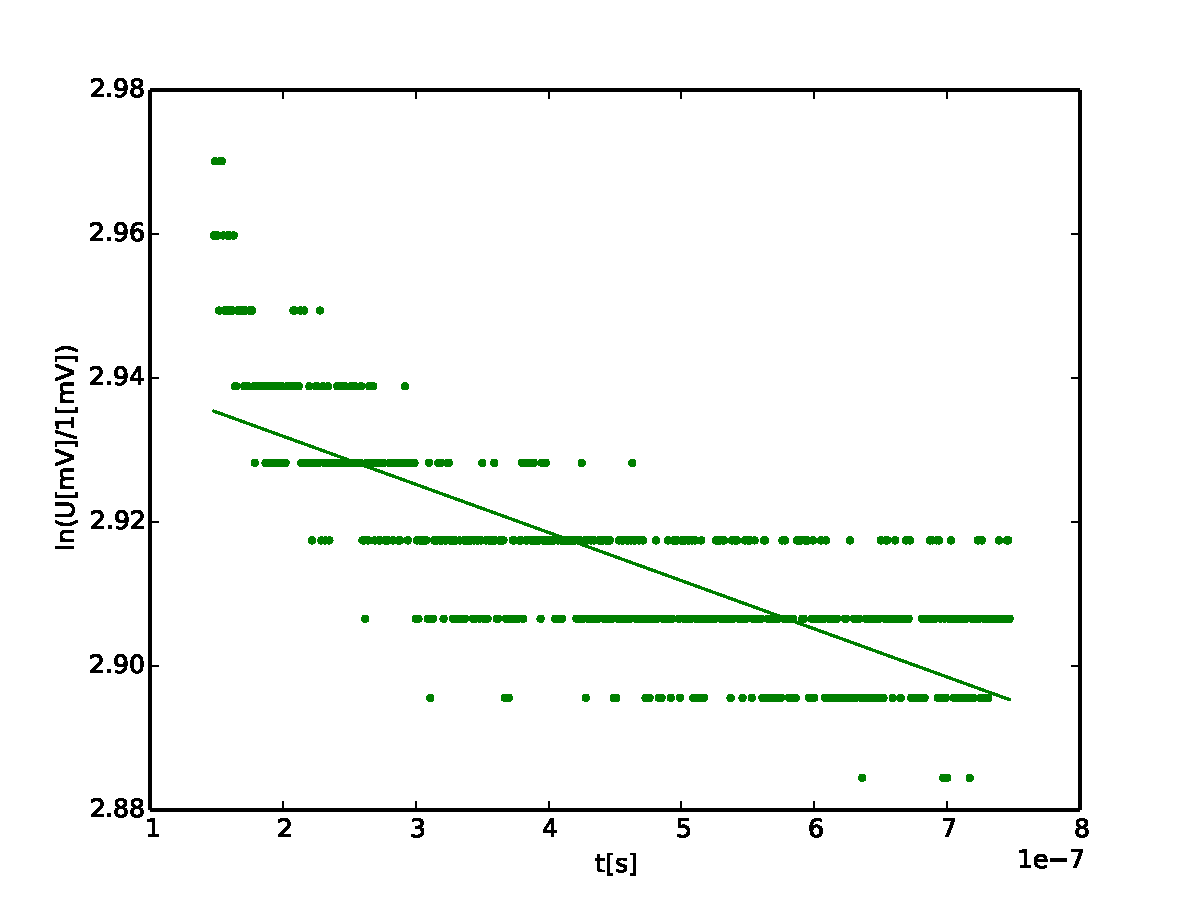
\includegraphics[width = 14cm]{data/d/Regression3.pdf}
	\caption{Lineare Ausgleichsrechnungen zur Bestimmung des Induktivbelages und des Kapazitivbelags.}
	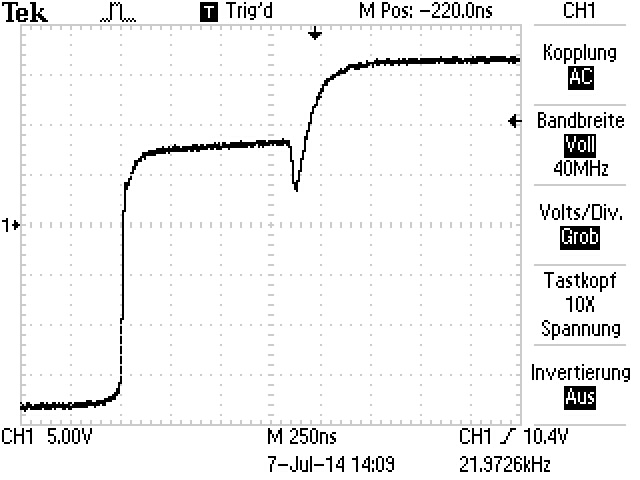
\includegraphics[width = 12cm]{data/d/F0007TEK.JPG}
	\caption{Spannungsverlauf von Abschluss 10.}
	\label{fig_abs10}
\end{figure}

\FloatBarrier
\subsection{E: Impulsfahrplan} % (fold)
\label{sub:subsection_name}

Um die Reflexionsfaktoren der Leitung zu erhalten, wird zunächst über die Spannungen jedes Plateaus gemittelt.
Anschließend wird von jedem Wert die Nullspannung $U_0$ abgezogen wodurch sich die Werte
\begin{eqnarray}
	U_0 &=& \SI{-23.32(5)}{\volt},\\
	U_1 &=& \SI{22.93(6)}{\volt},\\
	U_2 &=& \SI{28.87(6)}{\volt},\\
	U_3 &=& \SI{49.34(6)}{\volt},\\
	U_4 &=& \SI{46.76(7)}{\volt}
\end{eqnarray}
ergeben.

Als Differenz zwischen zwei aufeinanderfolgenden Spannungen ergiebt sich
\begin{eqnarray}
	\Delta U_1 = U_2 - U_1 &=& \SI{5.95(5)}{\volt},\\
	\Delta U_2 = U_3 - U_2 &=& \SI{20.46(5)}{\volt},\\
	\Delta U_3 = U_4 - U_3 &=& \SI{-2.58(6)}{\volt}.
\end{eqnarray}

Die Reflexionsfaktoren berechnen sich nach
\begin{eqnarray}
	\Gamma_L = \frac{\Delta U_1}{U_1} &=& \SI{0.2594(22)}{},\\
	\Gamma_E = \frac{\Delta U_3}{\Delta U_2} + \frac{\Delta U_2}{U_1(1-\Gamma_L)} &=& \SI{1.079(6)}{},\\
	\Gamma_R = \frac{\Delta U_3}{\Delta U_2 \Gamma_E} &=& \SI{-0.1168(28)}{}.
\end{eqnarray}

\begin{figure}
	\centering
	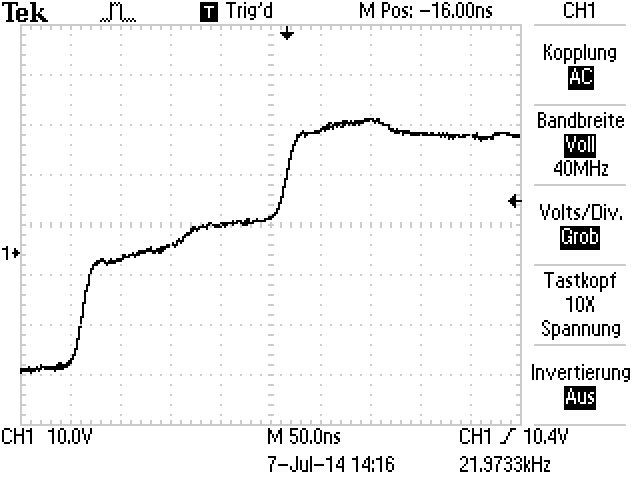
\includegraphics[width = 12cm]{data/e/ALL0008/F0008TEK.JPG}
	\caption{Spannungskurve einer Reihenschaltung von einem $\SI{50}{\ohm}$ und einem $\SI{75}{\ohm}$ Kabel.}
	\label{fig_abs10}
\end{figure}

\FloatBarrier
\section{Diskussion} % (fold)
\label{sec:diskussion}

Alles in allem lässt sich sagen, dass eine Signalübertragung mithilfe elektrischer Leitungen zu Problemen führen kann. 
So kann es zu Reflexionen oder anderen frequenzabhängigen Effekten kommen, welche berücksichtigt werden müssen.

Im ersten Teil konnten nur mit großer Mühe und Geduld hinreichende Messwerte aufgenommen werden, da das Messgerät Probleme mit dem erkennen des angeschlossenen Kabels hatte.
Es konnte jedoch gezeigt werden, dass der Induktivbelag $L$ und der Kapazitivbelag $C$ wie erwartet keine Frequenzabhängigkeit zeigt, während beim Widerstandsbelag $R$ und beim Querleitwertbelag $G$ eine Frequenzabhängigkeit zu erahnen ist.

Im zweiten Teil konnte gezeigt werden, dass die Dämpfungskonstante eines Kabels frequenzabhängig ist.

In Abschnitt C wurde festgestellt, dass eine Bestimmung der Kabellänge über eine Laufzeitmessung zu hinreichenden Ergebnissen führt.
Bei der Bestimmung mithilfe eines Smith-Diagramms kam es jedoch zu erheblichen Fehlern.
Dies könnte daran liegen, dass die idealisierten Annahmen zu fehlerhaften Größen führen.
Die Leitungskonstanten mithilfe der Spannungsverläufe zu bestimmen war gut möglich.

Abschnitt D zeigte, dass es möglich ist nur mithilfe der Spannungsverläufe auf die Art des Abschlusses zurückzuschließen.
Zudem ist es aus dem Spannungsverlauf möglich gewesen auf die Leitungskonstanten zurückzuschließen.

Abschließend konnte mithilfe des Spannungsverlaufs von in Reihe geschalteter Kabel ein Impulsfahrplan erzeugt werden.
Es lässt darauf schließen, dass mindestens eins der Kabel von seiner vorgegebenen Impedanz abweicht, da die Reflexionsfaktoren $\Gamma_L$ und $\Gamma_R$ betragsmäßig ungleich $0.2$ sind.

\section{Quellen} % (fold)
\label{sub:quellen}

[E02], author = Physikalisches Praktikum TU Dortmund,
  title = Versuch E2: Signale auf Leitungen, 
  howpublished = \url{http://129.217.224.2/HOMEPAGE/PHYSIKER/BACHELOR/FP/SKRIPT/Signale_E2.pdf},
  aufgerufen 2.7.2014

[koax], url{http://www.microwaves101.com/,
    aufgerufen September 2014
